\section{Задание 4. Приложение Рядов. Сиразетдинов Азат. Вариант 28}
\subsection{Задание 1}
Вычислить приближенно значение функции с точностью 0,0001 $ \cos48\degree $
\begin{eqnarray*} 
	&\text{Возьмем табличное разложение}\\
	&\cos x=  \sum_{k=0}^{\infty} (-1)^k \frac{x^{2k}}{(2k)!}\\
	&\cos48\degree = \cos(0,8378)\\
	&\text{1 член последовательности:}  \frac{0,8378^0}{1!} \approx 1\\
	&\text{2 член последовательности:}  (-1) * \frac{0,8378^2}{2!} \approx -0,35095\\
	&\text{3 член последовательности:}  \frac{0,8378^4}{4!} \approx 0,02052\\
	&\text{4 член последовательности:}  (-1) * \frac{0,8378^6}{6!} \approx -0,00048\\
	&\text{4 член последовательности:}  \frac{0,8378^8}{8!} \approx 0\\
	&\text{Дальнейшие члены не будут изменять точность}\\
	&\cos(0,8378) = 1 - 0,35095 + 0,02052 - 0,00048 \approx 0,66909 \approx 0,6691\\
\end{eqnarray*}
Проверка:
\begin{center}
	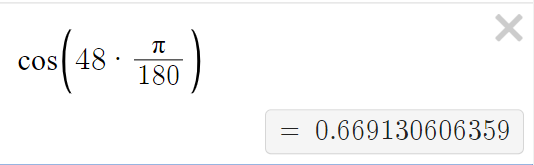
\includegraphics[width=.3\linewidth]{rgr2_task4_azat/cos_proof}\quad
\end{center}

